% A skeleton file for producing Computer Engineering reports
% https://kgcoe-git.rit.edu/jgm6496/KGCOEReport_template

\documentclass[CMPE]{../KGCOEReport}

% The following should be changed to represent your personal information
\newcommand{\classCode}{CMPE 460}  % 4 char code with number
\newcommand{\name}{Andrei Tumbar}
\newcommand{\LabSectionNum}{2}
\newcommand{\LabInstructor}{Beato}
\newcommand{\TAs}{Xavier Brooks\\
Diana Yakobchuk\\
Charles Poliwoda}
\newcommand{\exerciseNumber}{6}
\newcommand{\exerciseDescription}{PWM \& DC Motors \& Servo Motors}
\newcommand{\dateDone}{3/4/2022}
\newcommand{\dateSubmitted}{3/18/2022}
\newcommand{\LectureSectionNum}{1}
\newcommand{\LectureInstructor}{Beato}

\usepackage{tikz}
\usepackage{circuitikz}
\usetikzlibrary{calc}
\usepackage{multirow}
\usepackage{titlesec}
\usepackage{float}
\usepackage{lmodern}
\usepackage{pgfplots}
\usepackage{siunitx}
\usepackage{subcaption}
\usepackage{graphicx}
\usepackage[usestackEOL]{stackengine}
\usepackage{scalerel}
\usepackage[T1]{fontenc}
\usepackage{amsmath}
\usepackage{pdfpages}


\def\code#1{\texttt{#1}}

\begin{document}
    \maketitle
    \section*{Description}

   	This laboratory exercise looked at implementing drivers for three different
   	types of motors. The DC, servo and stepper motors. The DC motor operates by
   	simply passing current through the motor. The direction of current will
   	determine the direction that the motor will spin. The speed of a DC motor
   	may be controlled by pulsing the voltage across the two terminals at various
   	rates. The servo motor will hold its position given a PWM signal. Usually servo
   	motors will operate at a single PWM frequency and between a minimum and maximum
   	duty cycle. The duty cycles inside this range will control the position of the
   	servo motor. A stepper motor is a motor that will operate with multiple inductors
   	placed around the rotor. By pulsing these inductors in a certain order, the magnetic
   	field generated will cause the rotor to rotate by a certain amount. Stepper motors
   	may also be held in place in a closed loop fashion by providing active feedback
   	against a load to hold the rotor at a certain position. This makes stepper motors
   	a great choice for a kinematic robot that requires precise moving with high holding
   	torque.

    \section*{Wiring diagrams}
    \subsection*{DC motor}

	Because a DC motor will require a high amount of current that the microcontroller (MC)
	cannot viable provide, the DC motor must be isolated from the MC in
	a fashion that can also be controlled by the MC. To do this, an H-bridge array is
	used. The H-bridge array will allow the MC to switch the high voltage power supply
	(Vcc2) onto the motor terminals (1Y, 2Y).

	\begin{figure}[ht]
	  \centering
	  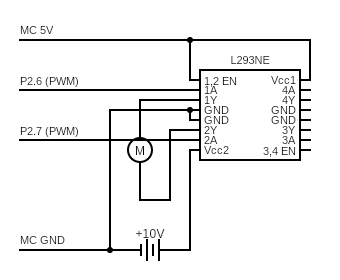
\includegraphics[width=.6\linewidth]{circuit}
	  \caption{DC Motor wiring.}
	  \label{fig:dc}
	\end{figure}

	Figure \ref{fig:dc} shows the wiring required to get the MC and the L293NE H-bridge
	array to control a DC motor. The inputs, 1A and 2A, will switch \SI{0}{\volt} or
	\SI{10}{\volt} onto their corresponding outputs, 1Y and 2Y, depending on the inputs
	logic level. To allow the motor to spin, one of the terminals should be raised to
	\SI{10}{\volt} while the other should be grounded to \SI{0}{\volt}. The speed of the
	motor can be controlled by pulsing the input line using a PWM signal. Varying the duty
	cycle will vary the resultant speed of the motor.\\

	Notice that Figure \ref{fig:dc} connects ground of the motor controller to the
	ground of the power supply. This will allow the reference voltage
	of the H-bridge logic (and output low) to match the ground on the power supply.
	The DC motor will not work without this connection.

	\subsection*{Stepper motor}

	Like the DC motor, the stepper motor requires current isolation between the micro
	controller and the motor coils. To achieve this, a Darlington array is used. A
	Darlinton array can act as a current amplifier which can power the each coil on
	stepper motor.

	\begin{figure}[ht]
	  \centering
	  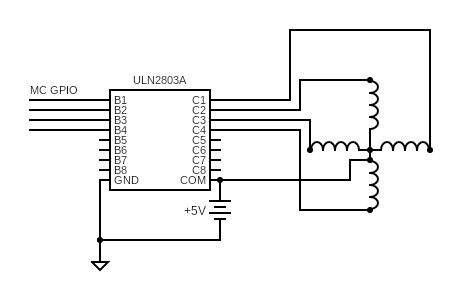
\includegraphics[width=.8\linewidth]{stepper}
	  \caption{Stepper Motor wiring.}
	  \label{fig:stepper}
	\end{figure}
	
	As shown in Figure \ref{fig:stepper}, a darlington array integrated circuit is
	controlled directly by GPIO pins on the MC. The common line is connected to an
	external power source and output pin is connected to the respective input terminal
	of the stepper motor's coil.

	\section*{Oscilloscope captures}

	Oscilloscope captures were taken for Parts 1 (Figure \ref{fig:cap1}) and 4
	(Figures

	\begin{figure}[ht]
		\centering
		 \begin{subfigure}[b]{0.4\textwidth}
		     \centering
		     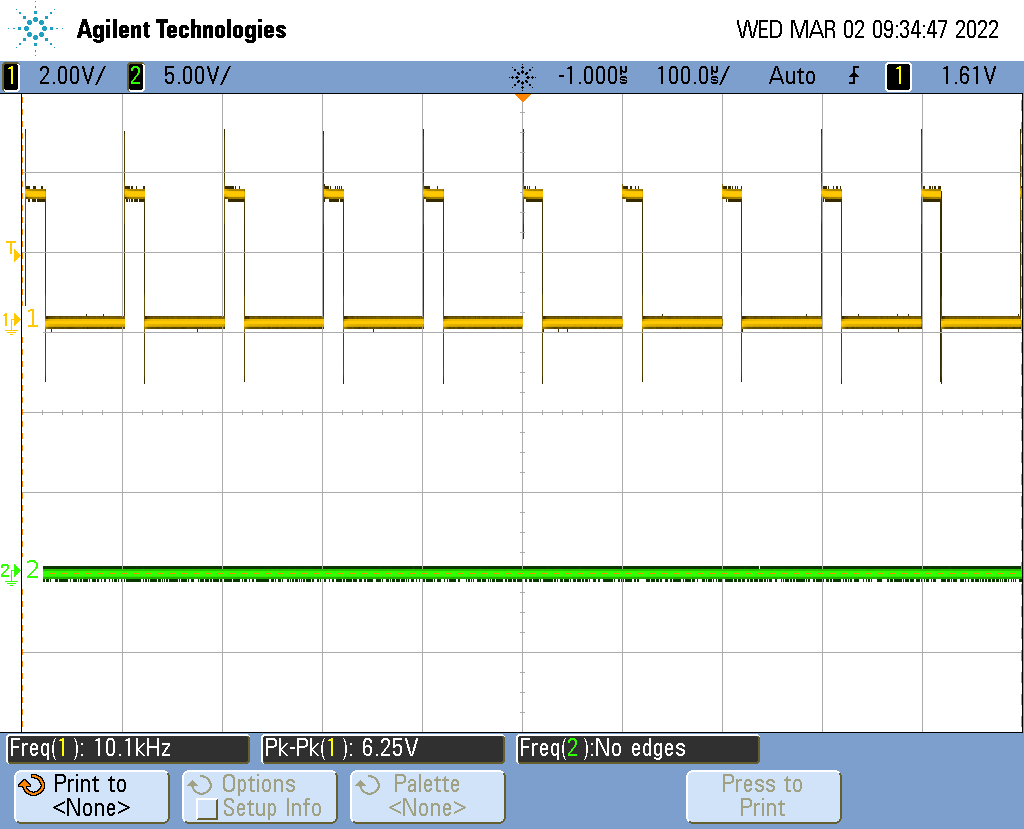
\includegraphics[width=\textwidth]{scope_0}
		     \caption{20\% duty cycle on \SI{10}{\kilo\hertz} PWM}
		     \label{fig:cap1}
		 \end{subfigure}
		 \hfill
		 \begin{subfigure}[b]{0.4\textwidth}
		     \centering
		     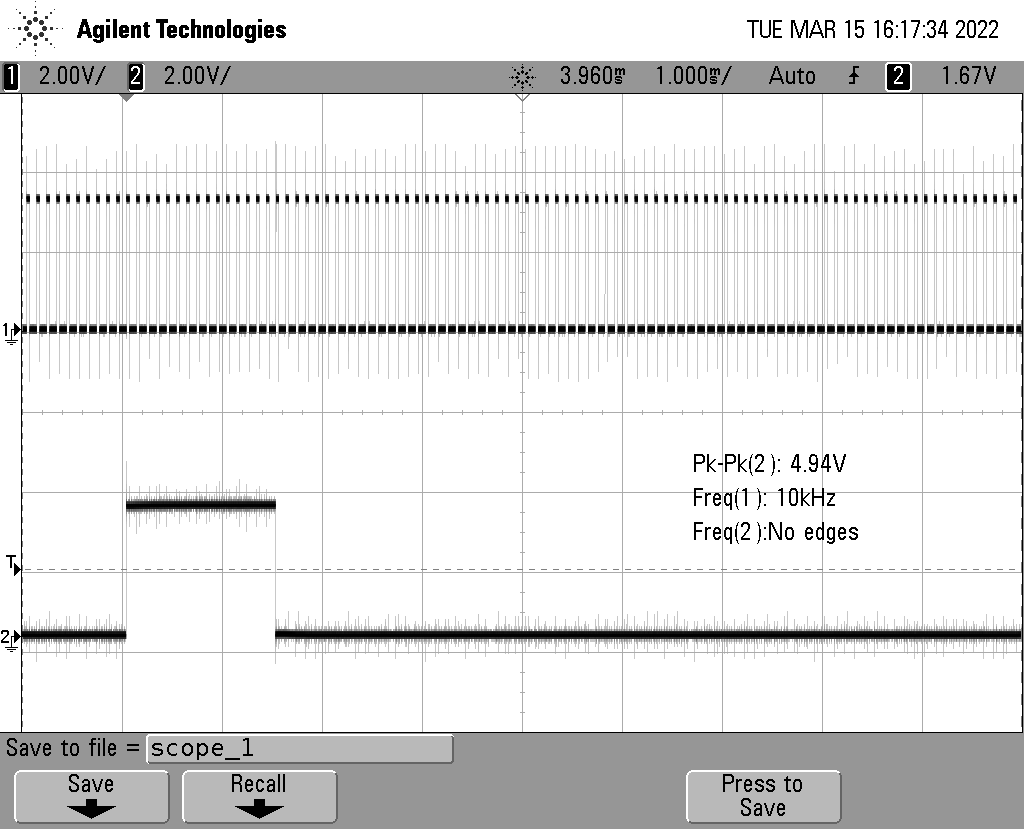
\includegraphics[width=\textwidth]{scope_1}
		     \caption{Left motor at 30\% (\SI{10}{\kilo\hertz}) and servo at 7.5\% (\SI{50}{\hertz}) simultaneously}
		     \label{fig:cap2}
		 \end{subfigure}
	\end{figure}

	\begin{figure}[ht]
		\centering
		 \begin{subfigure}[b]{0.4\textwidth}
		     \centering
		     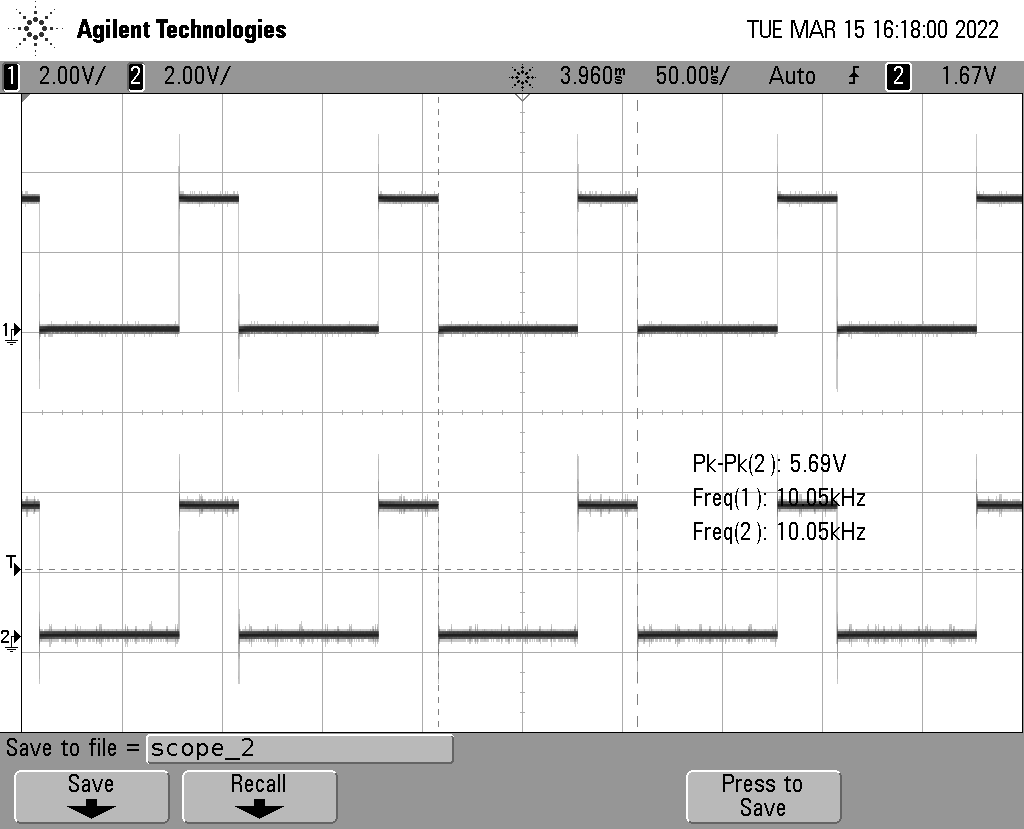
\includegraphics[width=\textwidth]{scope_2}
		     \caption{Left and right motor at 30\% (\SI{10}{\kilo\hertz}) simultaneously}
		     \label{fig:cap3}
		 \end{subfigure}
		 \hfill
		 \begin{subfigure}[b]{0.4\textwidth}
		     \centering
		     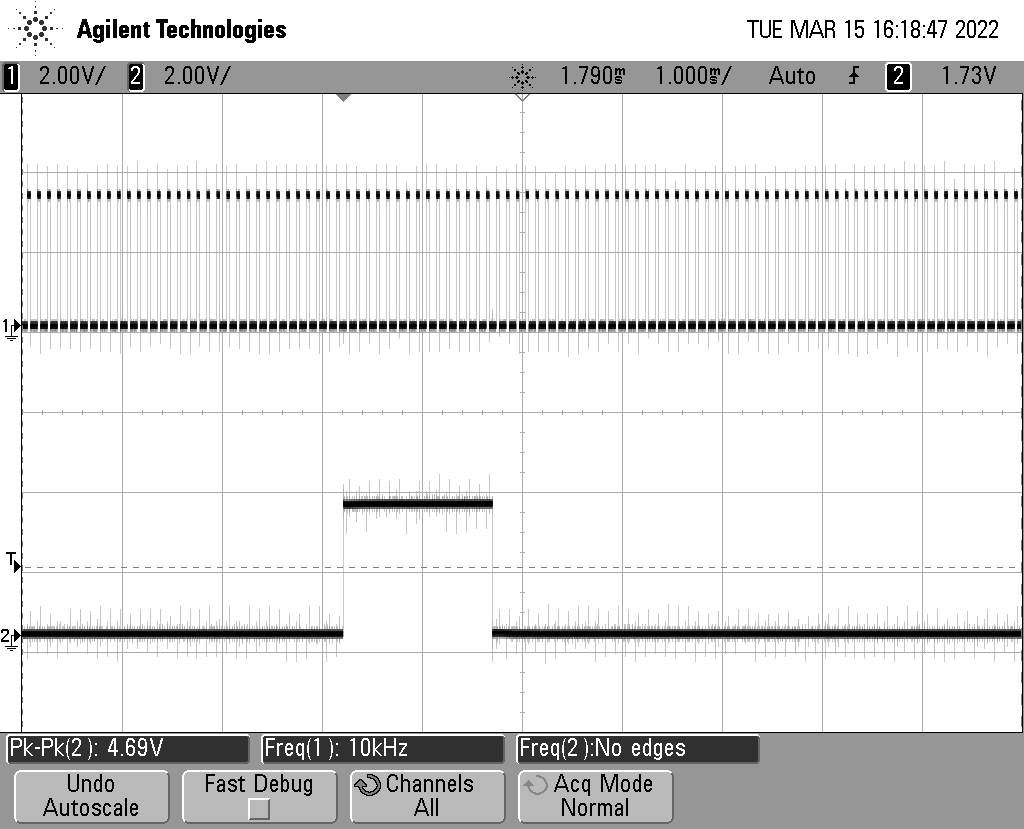
\includegraphics[width=\textwidth]{scope_3}
		     \caption{Right motor at 30\% (\SI{10}{\kilo\hertz}) and servo at 7.5\% (\SI{50}{\hertz}) simultaneously}
		     \label{fig:cap4}
		 \end{subfigure}
	\end{figure}

	\pagebreak
	\section*{Description of code}

	There are two new modules written to support the DC and servo motors. The \code{pwm}
	module will implement the lower level hardware configuration of the TimerA. This
	module supports all TimerA pins (TA0-3 5-pins per timer). Any of the PWM pins may
	be selected via a \code{PwmPin} object that will select both the timer and the pin
	on that timer. During initialization the base frequency of the timer channel can be
	configured. During runtime, the duty cycle may be set using a floating point number
	from \code{0.0} to \code{1.0}.\\

	The second module written to support this lab is the \code{dc} module. This module
	will simply wrap the \code{pwm} module to operate two pins, forward and backward.
	To control the direction and speed of the motor, a number between \code{-1.0} and
	\code{1.0} may be used where negative numbers will run the motor backward.\\

	To time the speedup and slowdown of the motor in part 2, a Timer32 was configured
	to interrupt at \SI{10}{\milli\s} intervals and increment a state counter. The
	state counter would count from 0 to 100 controlling the speed of the motor. Once
	overflown, the counter would reset and place the system into deceleration mode.
	The system oscillated between acceleration and deceleration modes until a switch
	press toggles to system to an OFF state.

	\section*{In-lab questions}

	\begin{enumerate}
	\item{Explain how to change speed and direction of turn of the DC motor.}

	The speed of the motor can be changed by varying the duty cycle of the PWM signal.
	The direction of the motor can be changed by swapping the terminals on the motor
	(or by feeding a PWM signal into the other terminal).

	\item{Describe in your lab report an alternate method in your report
	that uses only one PWM line and one GPIO line.}

	The PWM signal is connected to one terminal, the GPIO line to the other. To run
	the motor forward, drop the GPIO line to LOW and start the PWM signal with
	$duty\_cycle$. To run the
	motor backward, raise the GPIO line to HIGH and start the PWM signal with
	$1 - duty\_cycle$.

	\item{Which stepping mode does this code use?}

	Full-step (low torque)

	\end{enumerate}

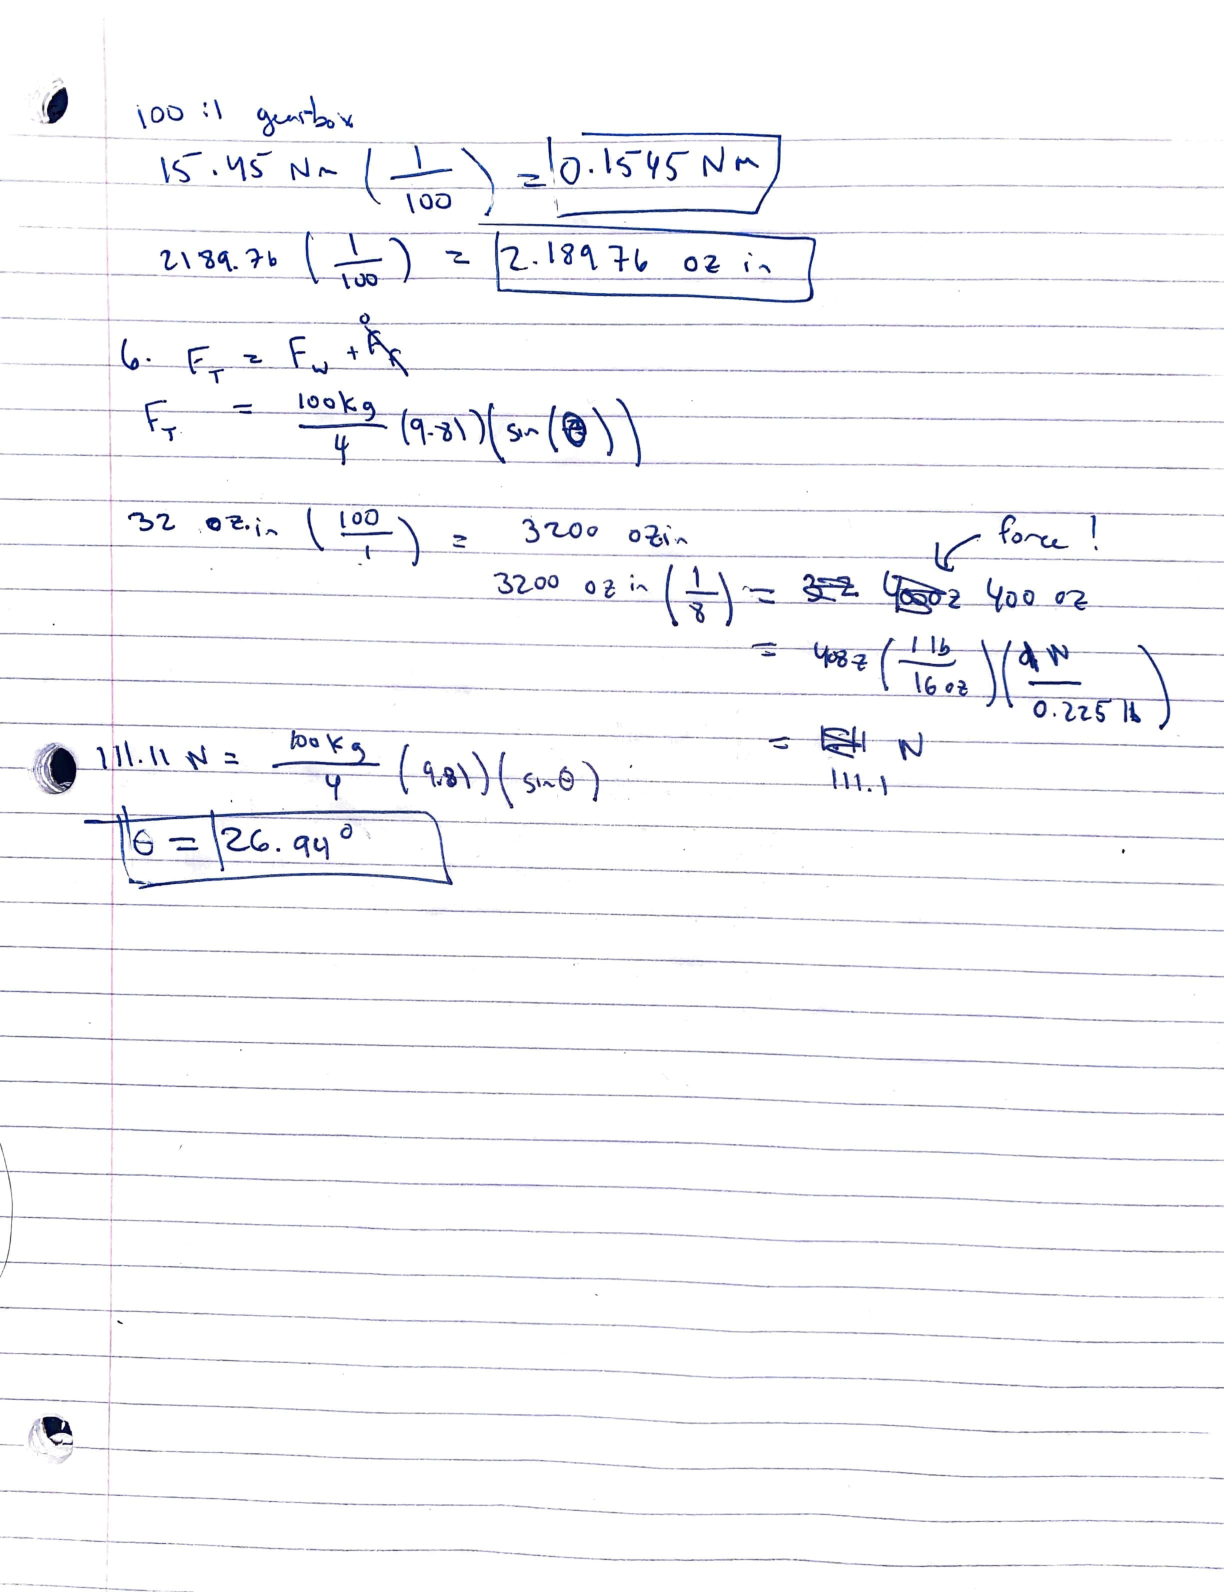
\includepdf[pages=-,pagecommand={},width=\textwidth]{prelab-and-signoff6.pdf}

\end{document}
